%%%%%%%%%%%%%%%%%%%%%%%%%%%%%%%%%%%%%%%%%%%%%%%%%%%%%%%%%%%%%%%%%%%%%
% LaTeX Template: Project Titlepage Modified (v 0.1) by rcx
%
% Original Source: http://www.howtotex.com
% Date: February 2014
% 
% This is a title page template which be used for articles & reports.
% 
% This is the modified version of the original Latex template from
% aforementioned website.
% 
%%%%%%%%%%%%%%%%%%%%%%%%%%%%%%%%%%%%%%%%%%%%%%%%%%%%%%%%%%%%%%%%%%%%%%

\documentclass[11pt]{article}
%\usepackage[a4paper]{geometry}
\usepackage[left=1.5cm,right=1.5cm,top=2cm,bottom=2cm]{geometry}
\setlength\parindent{0pt}
\setlength{\parskip}{1em}
\usepackage[table,xcdraw]{xcolor}
\usepackage{fancyhdr}
\usepackage{helvet}
\usepackage{lastpage}
\usepackage{graphicx, wrapfig, setspace, booktabs}
\usepackage{titlepic}
\usepackage[T1]{fontenc}
\usepackage[font=small, labelfont=bf,center]{caption}
\usepackage{fourier}
\usepackage[protrusion=true, expansion=true]{microtype}
\usepackage[english]{babel}
\usepackage{sectsty}
\usepackage{url, lipsum}
\usepackage{multirow}
\usepackage{float}
\usepackage{amsmath}
\usepackage{bm}
\usepackage{subfig}
\usepackage{tikz}
\usepackage{svg}
\usepackage[final]{pdfpages}
\usepackage{hyperref}
\usepackage[all]{hypcap}
\newcommand{\HRule}[1]{\rule{\linewidth}{#1}}
\onehalfspacing
\setcounter{tocdepth}{5}
\setcounter{secnumdepth}{5}

%-------------------------------------------------------------------------------
% HEADER & FOOTER
%-------------------------------------------------------------------------------
\pagestyle{fancy}
\fancyhf{}
\setlength\headheight{15pt}
\fancyhead[L]{iz16368}
\fancyhead[R]{University of Bristol}
\fancyfoot[R]{Page \thepage\ of \pageref{LastPage}}
%-------------------------------------------------------------------------------
% TITLE PAGE
%-------------------------------------------------------------------------------

\begin{document}

\title{ \normalsize \textsc{Advanced Space Systems}
		\\ [2.0cm]
		\HRule{0.5pt} \\
		\LARGE \textbf{\uppercase{New Horizons GMAT Coursework}}
		\HRule{2pt} \\ [0.5cm]
		\normalsize \today \vspace*{5\baselineskip}}

\date{}

% \titlepic{\includegraphics[width=0.8\textwidth]{QUANSER.png}}

\author{
		Ismaeel Zaman  \\ 
		\\
		University of Bristol \\
		Department of Aerospace Engineering }

\maketitle
\thispagestyle{empty}
\newpage
% \tableofcontents
% \thispagestyle{empty}
% \newpage
% \listoftables
% \thispagestyle{empty}
% \listoffigures
% \thispagestyle{empty}
% \newpage
\setcounter{page}{1}
%-------------------------------------------------------------------------------
% Section title formatting
%\sectionfont{\scshape}
%-------------------------------------------------------------------------------

%-------------------------------------------------------------------------------
% BODY
%-------------------------------------------------------------------------------
\includepdf[landscape=true, pages=2]{ASSCW.pdf}


\newpage

\section{Mission Overview}

% 1. A brief explanation, using diagrams, of the timeline of the mission you chose, starting
% from Earth departure. Please ensure that you label your figures and tables and cite any
% references that you use.\\

New Horizons, as seen in the diagram above, is an interplanetary mission with the primary goal of performing a flyby study of the dwarf planet Pluto and secondary mission to study an element of the Kuiper Belt known as Ultima Thule. \\

The New Horizons space probe was launched from Cape Canaveral on 19$^{th}$ January 2006 immediately into an Earth-and-Solar escape trajectory. It would use a significant gravity assist from Jupiter in order to conserve fuel and to reduce mission duration. During the long period of uninterrupted flight the spacecraft was sent into deep sleep, waking only annually for systems checks.
A detailed mission timeline can be seen below:


\begin{table}[H]
\centering
\caption{Table showing Mission Timeline}
\begin{tabular}{@{}cll@{}}
\toprule
\rowcolor[HTML]{CBCEFB} 
\begin{tabular}[c]{@{}c@{}}Modified Julian\\ Date\end{tabular} & \multicolumn{1}{c}{\cellcolor[HTML]{CBCEFB}\begin{tabular}[c]{@{}c@{}}UTC Gregorian \\ Date\end{tabular}} & \multicolumn{1}{c}{\cellcolor[HTML]{CBCEFB}Event} \\ \midrule
\rowcolor[HTML]{DEFFDE} 
23755                                                          & 19th January 2006                                                                                         & Launch from Cape Canaveral                        \\
\rowcolor[HTML]{DEFFDE} 
23756                                                          & 20th January 2006                                                                                         & Leave Earth SOI                                   \\
\rowcolor[HTML]{DEFFDE} 
23804                                                          & 9th March 2006                                                                                            & TCM-1                                             \\
\rowcolor[HTML]{F5FFA2} 
24130                                                          & 29th January 2007                                                                                         & Enter Jupiter SOI                                 \\
\rowcolor[HTML]{F5FFA2} 
24160                                                          & 28th February 2007                                                                                        & Jupiter Periapsis                                 \\
\rowcolor[HTML]{F5FFA2} 
24189                                                          & 30th March 2007                                                                                           & Leave Jupiter SOI                                 \\
\rowcolor[HTML]{F5FFA2} 
24369                                                          & 25th September 2007                                                                                       & TCM - 2                                           \\
\rowcolor[HTML]{FFD8AD} 
27218                                                          & 14th July 2015                                                                                            & Pluto flyby                                       \\
\rowcolor[HTML]{FFD8AD} 
27297                                                          & 1st October 2015                                                                                          & TCM-3                                             \\
\rowcolor[HTML]{FFB3B3} 
28485                                                          & 1st January 2019                                                                                          & Ultima Thule flyby                                     \\ \bottomrule
\end{tabular}
\label{tab:timeline}
\end{table}

The Trajectory Corrections were performed as early as possible in each manoeuvre so as to reduce fuel consumption.
During the long period of uninterrupted flight the spacecraft was sent into deep sleep, waking only annually for systems checks.


\section{Model Mission Sequence}
2. A ‘copy-paste’ of the ‘mission sequence’ of your model and provide a discussion of this,
including descriptions of each stage as well as a discussion of why you have chosen to
model the mission this way and the values you have chosen. Include any simplifications
or assumptions you have made.
[20 marks]\\

\begin{figure}[H]
    \centering
    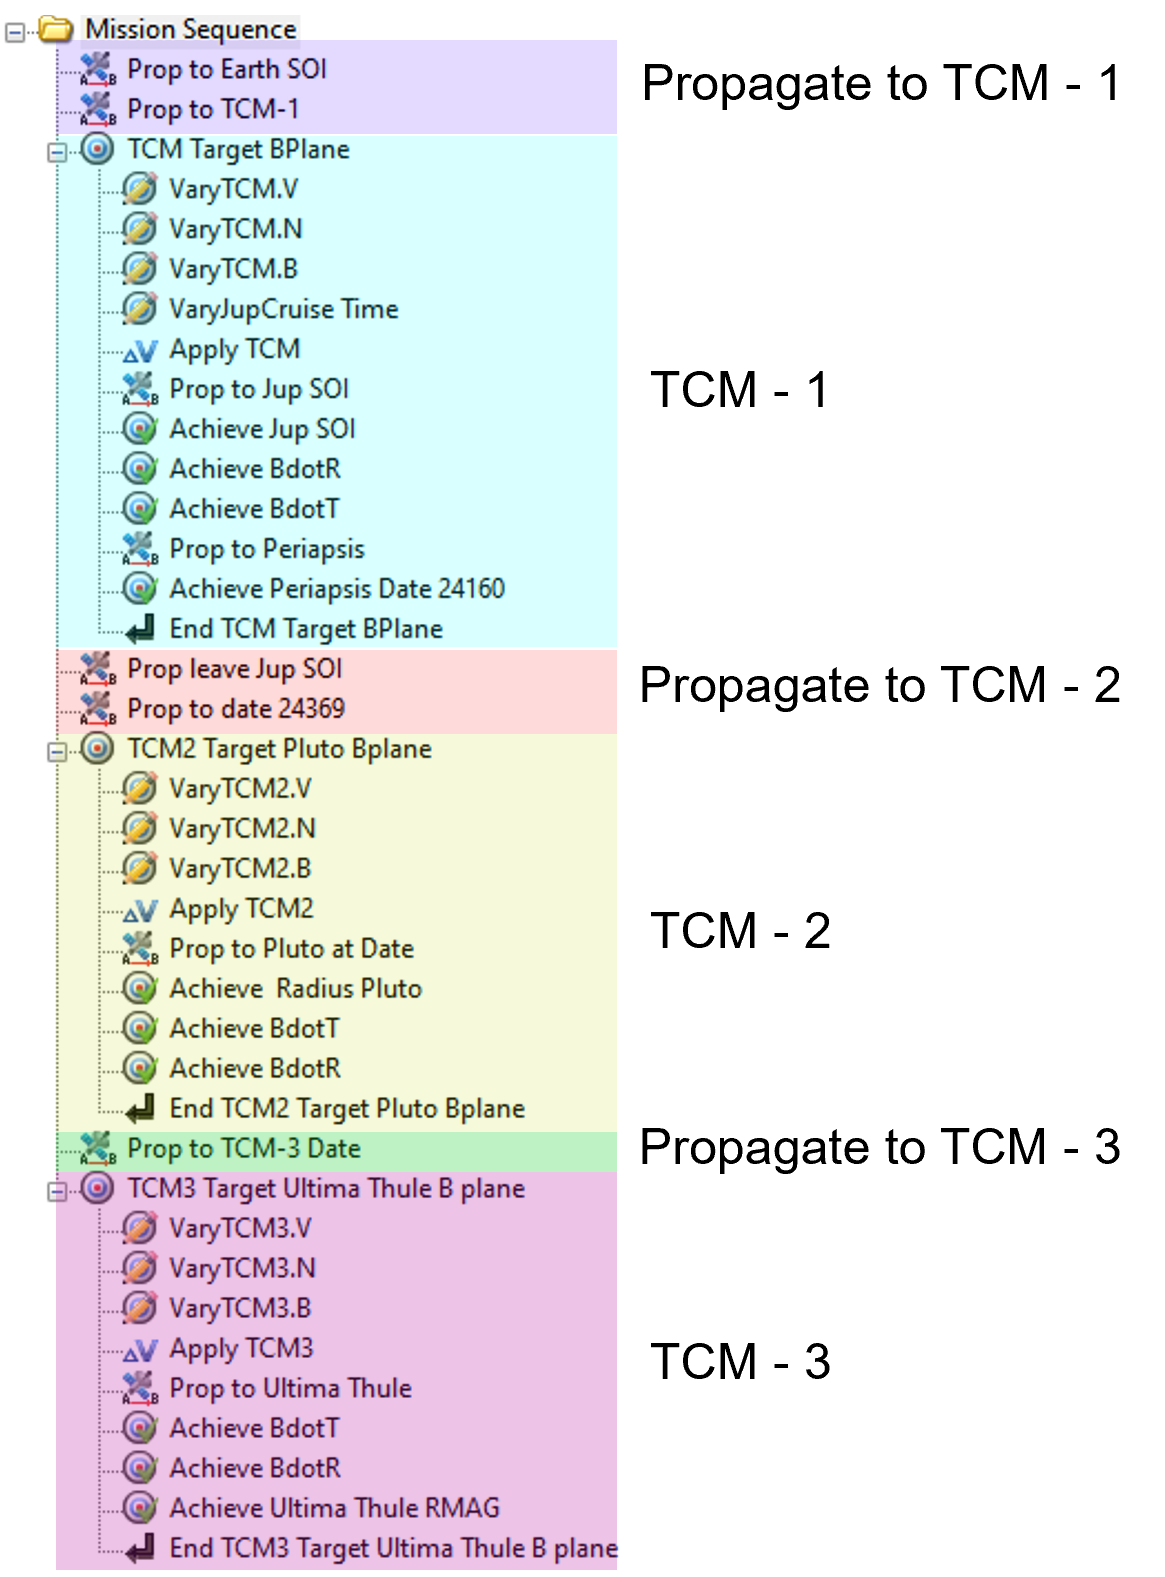
\includegraphics[width=0.6\textwidth]{Mission.PNG}
    \caption{Caption}
    \label{fig:my_label}
\end{figure}

\textbf{Propagate to TCM - 1} This section serves to propagate the spacecraft 


\section{Discussion}
3. A discussion of assumptions that GMAT makes when modelling interplanetary missions.
[20 marks]\\

Assumptions:
\begin{itemize}
    \item Point Masses
    \item Burns are instantaneous impulses
    \item No Mass decrement
\end{itemize}





4. Compare the results of your model to the actual mission, how do delta Vs, distances,
times, etc. differ and why?
[20 marks]






%-------------------------------------------------------------------------------
% REFERENCES
%-------------------------------------------------------------------------------

%-------------------------------------------------------------------------------
% APPENDIX
%-------------------------------------------------------------------------------
\appendix
%\addcontentsline{toc}{section}{APPENDIX}
\renewcommand\thefigure{A.\arabic{figure}}  
\setcounter{figure}{0}



\end{document}




%-------------------------------------------------------------------------------
% SNIPPETS
%-------------------------------------------------------------------------------

% \begin{figure}[!ht]
% 	\centering
% 	\includegraphics[width=0.8\textwidth]{file_name}
% 	\caption{}
% 	\centering
% 	\label{label:file_name}
% \end{figure}

%\begin{figure}[!ht]
%	\centering
%	\includegraphics[width=0.8\textwidth]{graph}
%	\caption{Blood pressure ranges and associated level of hypertension (American Heart Association, 2013).}
%	\centering
%	\label{label:graph}
%\end{figure}

%\begin{wrapfigure}{r}{0.30\textwidth}
%	\vspace{-40pt}
%	\begin{center}
%		\includegraphics[width=0.29\textwidth]{file_name}
%	\end{center}
%	\vspace{-20pt}
%	\caption{}
%	\label{label:file_name}
%\end{wrapfigure}

%\begin{wrapfigure}{r}{0.45\textwidth}
%	\begin{center}
%		\includegraphics[width=0.29\textwidth]{manometer}
%	\end{center}
%	\caption{Aneroid sphygmomanometer with stethoscope (Medicalexpo, 2012).}
%	\label{label:manometer}
%\end{wrapfigure}

%\begin{table}[!ht]\footnotesize
%	\centering
%	\begin{tabular}{cccccc}
%	\toprule
%	\multicolumn{2}{c} {Pearson's correlation test} & \multicolumn{4}{c} {Independent t-test} \\
%	\midrule	
%	\multicolumn{2}{c} {Gender} & \multicolumn{2}{c} {Activity level} & \multicolumn{2}{c} {Gender} \\
%	\midrule
%	Males & Females & 1st level & 6th level & Males & Females \\
%	\midrule
%	\multicolumn{2}{c} {BMI vs. SP} & \multicolumn{2}{c} {Systolic pressure} & \multicolumn{2}{c} {Systolic Pressure} \\
%	\multicolumn{2}{c} {BMI vs. DP} & \multicolumn{2}{c} {Diastolic pressure} & \multicolumn{2}{c} {Diastolic pressure} \\
%	\multicolumn{2}{c} {BMI vs. MAP} & \multicolumn{2}{c} {MAP} & \multicolumn{2}{c} {MAP} \\
%	\multicolumn{2}{c} {W:H ratio vs. SP} & \multicolumn{2}{c} {BMI} & \multicolumn{2}{c} {BMI} \\
%	\multicolumn{2}{c} {W:H ratio vs. DP} & \multicolumn{2}{c} {W:H ratio} & \multicolumn{2}{c} {W:H ratio} \\
%	\multicolumn{2}{c} {W:H ratio vs. MAP} & \multicolumn{2}{c} {\% Body fat} & \multicolumn{2}{c} {\% Body fat} \\
%	\multicolumn{2}{c} {} & \multicolumn{2}{c} {Height} & \multicolumn{2}{c} {Height} \\
%	\multicolumn{2}{c} {} & \multicolumn{2}{c} {Weight} & \multicolumn{2}{c} {Weight} \\
%	\multicolumn{2}{c} {} & \multicolumn{2}{c} {Heart rate} & \multicolumn{2}{c} {Heart rate} \\
%	\bottomrule
%	\end{tabular}
%	\caption{Parameters that were analysed and related statistical test performed for current study. BMI - body mass index; SP - systolic pressure; DP - diastolic pressure; MAP - mean arterial pressure; W:H ratio - waist to hip ratio.}
%	\label{label:tests}
%\end{table}
